\begin{savequote}[45mm]
\ascii{Any fool can write code that a computer can understand. Good programmers write code that humans can understand.}
\qauthor{\ascii{- Martin Flower}}
\end{savequote}

\chapter{隐式树} 
\label{ch:implicit-tree}

\begin{content}

\end{content}

\section{测试套件}

\begin{content}

如果每个用例都需要手动地执行\ascii{run},显得极其笨拙。可以将一堆测试用例打包,用一个简单的\ascii{for}循环依次执行每个用例。

\subsection{测试用例}

为了确定每个\ascii{TestCase}都被执行,可以简单定制一个计数器\ascii{num}。用例执行后,断言已运行用例的数目。

\begin{nodiff}{test/mars/core/TestSuiteSpec.cc}
 \begin{c++}
#include <gtest/gtest.h>
#include "mars/core/TestCase.h"
#include "mars/core/TestSuite.h"

namespace {
  int num = 0;

  struct FooTest : TestCase {
  private:
    void runTest() override {
      num++;
    }
  };
}

TEST(TestSuite, pack_test_cases_into_test_suite) {
  TestSuite suite;
  suite.add(new FooTest);
  suite.add(new FooTest);

  suite.run();

  ASSERT_EQ(2, num);
}
 \end{c++}
\end{nodiff}

\subsection{通过编译}

为了快速通过编译,创建\ascii{TestSuite}的头文件。需要注意的是,\ascii{TestSuite}仅对\ascii{TestCase}的指针类型产生依赖,前置声明\ascii{struct TestCase}即可。但是,\ascii{TestSuite}对值对象\ascii{std::vector}则表现为强依赖,因此需要包含头文件。

\begin{nodiff}{include/mars/core/TestSuite.h}
 \begin{c++}
#include <vector>

struct TestCase;

struct TestSuite {
  void add(TestCase* test);
  void run();

private:
  std::vector<TestCase*> tests;
};
 \end{c++}
\end{nodiff}

\begin{episode}{最小化编译时依赖: 前置声明 VS. 包含头文件}

\begin{content}

当头文件中仅对类的声明产生依赖,那么前置声明是一种有效降低编译时依赖的重要技术。相反,头文件包含了本不应该包含的头文件,其编译时依赖将被间接污染到其他文件中,重编译将成为大概率事件。

在包含头文件还是前置声明抉择中,其依据的规则其实非常简单。在如下场景前置声明即可,无需包含头文件。

\begin{enum}
  \eitem{\ascii{指针}}
  \eitem{\ascii{引用}}
  \eitem{\ascii{返回值}}
  \eitem{\ascii{函数参数}}
\end{enum}

但是,如果编译器需要知道实体的确切内容,包括类的大小、布局、值等强编译时依赖信息,则必须包含头文件。强编译时依赖包括如下几种场景。

\begin{enum}
  \eitem{\ascii{继承}}
  \eitem{\ascii{宏}}
  \eitem{\ascii{inline}}
  \eitem{\ascii{template}}
  \eitem{\ascii{引用类内部成员时}}
  \eitem{\ascii{值类型的类成员变量}}  
  \eitem{执行\ascii{sizeof}运算}  
  \eitem{\ascii{typedef/using}类型别名}
\end{enum}

\end{content}

\end{episode}

\subsection{通过测试}

为了通过测试,可以快速实现\ascii{TestSuite::run}的逻辑。

\begin{nodiff}{src/mars/core/TestSuite.cc}
 \begin{c++}
#include "mars/core/TestSuite.h"
#include "mars/core/TestCase.h"

void TestSuite::add(TestCase* test) {
  tests.push_back(test);
}

void TestSuite::run() {
  for (auto test : tests) {
    test->run();
  }
}
 \end{c++}
\end{nodiff}

\begin{episode}{验证头文件的自满足性}

\begin{content}

所谓头文件自满足性,即头文件自身是可编译成功的。为了验证头文件的自满足性,其实现文件需要第一个包含对应的头文件。如果此头文件不自满足,自然会导致编译失败,此方法是验证头文件是否自满足的一个有效方法。

例如,对于头文件\ascii{include/mars/core/TestSuite.h},在其相应的实现文件中,需要第一个包含自己的头文件。

\begin{inlinediff}
 \begin{minicpp}
// 反例
#include "mars/core/TestCase.h"
#include "mars/core/TestSuite.h"
 \end{minicpp} 
\tcblower
 \begin{minicpp}
// 正例
#include "mars/core/TestSuite.h"
#include "mars/core/TestCase.h"
 \end{minicpp} 
\end{inlinediff}

头文件作为代码所有者对外公开\ascii{API}的重要途径。在发布之前,有责任保证其可用性,及其最小依赖性。如果一个头文件不自满足,当客户需要引用该头文件时,则需要客户自行承担寻找相关依赖的职责。客户因缺乏相关上下文信息,寻找缺失的依赖并非易事。

在极端条件下,头文件可能不存在相应的实现文件。例如,模板类或模板函数。此时,可以创建相应的测试文件,第一个包含其对应的头文件,校验头文件的自满足性;并对该模板实例化,实施简单的测试,确保编译与功能正确。

\begin{c++}[title={\ttfamily{实现ScopedExit:include/mars/util/ScopedExit.h}}]
#include "mars/util/Symbol.h"

template <typename F>
struct ScopedExit {
  ScopedExit(F f) : f(f) {
  }

  ~ScopedExit(){ 
    f(); 
  }

private:
  F f;
};

template <typename F>
ScopedExit<F> make_scoped_exit(F f) {
  return ScopedExit<F>(f);
};

#define SCOPED_EXIT(f) \
    auto UNIQUE_NAME(scoped_exit_) = make_scoped_exit(f)
\end{c++}

其中,\ascii{UNIQUE\_NAME}是一个通用的宏,可以放在基础设施之中。

\begin{c++}[title={\ttfamily{实用宏:include/mars/util/Symbol.h}}]
#define __DO_JOIN_AGAIN(symbol1, symbol2) symbol1##symbol2
#define __DO_JOIN(symbol1, symbol2) __DO_JOIN_AGAIN(symbol1, symbol2)

#define JOIN(symbol1, symbol2) __DO_JOIN(symbol1, symbol2)
#define UNIQUE_NAME(prefix) JOIN(prefix, __COUNTER__)
\end{c++}

在测试文件中,第一个包含该头文件,并尝试最简单的单元测试。

\begin{c++}[title={\ttfamily{测试ScopedExit:test/mars/util/ScopedExitSpec.cc}}]
#include "mars/util/ScopedExit.h"
#include <gtest/gtest.h>
#include <stdio.h>

TEST(ScopedExitSpec, close_file_safely) {
  auto file = std::fopen("~/.bashrc", "r");
  SCOPED_EXIT([file] {
    fclose(file);
  });
}
\end{c++}

\end{content}

\end{episode}

\subsection{内存泄露}

\ascii{TestSuite}持有若干\ascii{TestCase}实例,引入析构函数释放动态创建并添加至\ascii{TestSuite}的所有\ascii{TestCase}实例。

\begin{diff}{include/mars/core/TestSuite.h}
 \begin{minicpp}
#include <vector>

struct TestCase;

struct TestSuite {
  void add(TestCase* test);
  void run();

private:
  std::vector<TestCase*> tests;
};
 \end{minicpp}
\tcblower
 \begin{minicpp}
#include <vector>

struct TestCase;

struct TestSuite {
  ~TestSuite();

  void add(TestCase* test);
  void run();

private:
  std::vector<TestCase*> tests;
};
 \end{minicpp}
\end{diff}

实现析构函数,释放动态内存。

\begin{diff}{src/mars/core/TestSuite.cc}
 \begin{minicpp}
#include "mars/core/TestSuite.h"
#include "mars/core/TestCase.h"

void TestSuite::add(TestCase* test) {
  tests.push_back(test);
}

void TestSuite::run() {
  for (auto test : tests) {
    test->run();
  }
}
 \end{minicpp}
\tcblower
 \begin{minicpp}
#include "mars/core/TestSuite.h"
#include "mars/core/TestCase.h"

TestSuite::~TestSuite() {
  for (auto test : tests) {
    delete test;
  }
}

void TestSuite::add(TestCase* test) {
  tests.push_back(test);
}

void TestSuite::run() {
  for (auto test : tests) {
    test->run();
  }
}
 \end{minicpp}
\end{diff}

\subsection{消除重复}

为了消除析构函数与\ascii{run}之间的重复代码,提取一个公共的\ascii{foreach}函数。注意,不要在头文件直接实现该模板函数,最小化编译时的依赖。

\begin{diff}{include/mars/core/TestSuite.h}
 \begin{minicpp}
#include <vector>

struct TestCase;

struct TestSuite {
  ~TestSuite();

  void add(TestCase* test);
  void run();

private:
  std::vector<TestCase*> tests;
};
 \end{minicpp}
\tcblower
 \begin{minicpp}
#include <vector>

struct TestCase;

struct TestSuite {
  ~TestSuite();

  void add(TestCase* test);
  void run();

private:
  template <typename F>
  void foreach(F f) const;

private:
  std::vector<TestCase*> tests;
};
 \end{minicpp}
\end{diff}

可以使用\ascii{Lambda}表达式定制各种算子,实现差异化配置,实现对迭代算法的高度复用。

\begin{diff}{src/mars/core/TestSuite.cc}
 \begin{minicpp}
#include "mars/core/TestSuite.h"
#include "mars/core/TestCase.h"

TestSuite::~TestSuite() {
  for (auto test : tests) {
    delete test;
  }
}

void TestSuite::add(TestCase* test) {
  tests.push_back(test);
}

void TestSuite::run() {
  for (auto test : tests) {
    test->run();
  }
}
 \end{minicpp}
\tcblower
 \begin{minicpp}
#include "mars/core/TestSuite.h"
#include "mars/core/TestCase.h"

void TestSuite::add(TestCase* test) {
  tests.push_back(test);
}

template <typename F>
inline void TestSuite::foreach(F f) const {
  for (auto test : tests) {
    f(test);
  }
}

TestSuite::~TestSuite() {
  foreach([](auto test) {
    delete test;
  });
}

void TestSuite::run() {
  foreach([](auto test) {
    test->run();
  });
}
 \end{minicpp}
\end{diff}

设计分离了两个变化方向,使其两者完全分离,并能独立变化。

\begin{enum}
  \eitem{\ascii{迭代算法:因存储结构变化而变化(目前实现为线性表);}}
  \eitem{\ascii{处理算子:存在删除,计数,运行等操作。}}
\end{enum}

\begin{episode}{基于范围的for语句}

\begin{content}

存在泛型方法\ascii{foreach}的一种实现。不幸的是,它引入了复杂的\ascii{typedef typename}类型别名机制\footnote{\cpp{}也因诸如此类冗余的、复杂的类型说明,招致不公平的评论。}。

 \begin{c++}[title={\ttfamily{实现foreach:应用for循环,C++98}}]
template<typename T, typename F>
void foreach(const std::vector<T>& c, F f) {
  typedef typename std::vector<T>::const_iterator Iterator;
  for (Iterator first = c.begin(), last = c.end(); first != last; ++first) {
    f(*first);
  }
}
 \end{c++}

得益于\ascii{C++11}自动类型推演,可以去除\ascii{typedef}类型别名。

 \begin{c++}[title={\ttfamily{实现foreach:应用for循环,auto类型推演,C++11}}]
template<typename T, typename F>
void foreach(const std::vector<T>& c, F f) {
  for (auto first = c.begin(), last = c.end(); first != last; ++first) {
    f(*first);
  }
}
 \end{c++}

甚至,可以使用基于范围的\ascii{for}语句替代常规的\ascii{for}循环。

 \begin{c++}[title={\ttfamily{实现foreach:应用基于范围的\ascii{for},C++11}}]
template<typename T, typename F>
void foreach(const std::vector<T>& c, F f) {
  for (const T& e : c) {
    f(e);
  }
}
 \end{c++}

可以将\ascii{auto}实施到底,\ascii{foreach}实现变得更加简单、实用。

 \begin{c++}[title={\ttfamily{实现foreach:应用基于范围的\ascii{for},auto类型推演,C++11}}]
template<typename T, typename F>
void foreach(const std::vector<T>& c, F f) {
  for (const auto& e : c) {
    f(e);
  }
}
 \end{c++}

遗憾的是,\ascii{foreach}不够泛型,它只能接受\ascii{std::vector},而不能接受其他容器类型,例如\ascii{std::list, std::deque, std::set}。重构\ascii{foreach}接口,使其容器类型完全泛型化,甚至能够接受临时对象\footnote{因为容器类型使用的是\ascii{const}引用类型。}。

 \begin{c++}[title={\ttfamily{实现foreach:容器泛化,C++11}}]
template<typename Container, typename F>
void foreach(const Container& c, F f) {
  for (const auto& e : c) {
    f(e);
  }
}
 \end{c++}

\end{content}

\end{episode}

\section{嵌套结构}

为了实现更好的可扩展性,\ascii{TestSuite}不仅能打包\ascii{TestCase}实例,也应该能够打包更小的\ascii{TestSuite}的子实例,实现隐式的树结构。如\refig{test-case-tree}所示。

\begin{figure}
\centering
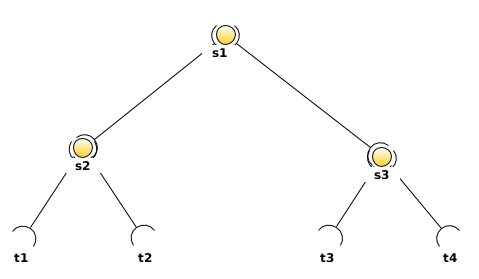
\includegraphics[width=0.8\textwidth]{figures/xunit/test-tree-example.png}
\caption{用例树:TestSuite(s1, s2, s3),TestCase(t1,t2,t3,t4)}
 \label{fig:test-case-tree}
\end{figure}

\subsection{测试依赖}

当执行用例时,确保\ascii{num}被初始化为\ascii{0};否则测试用例之间存在数据脏写的错误依赖。经过重构,\ascii{num}在\ascii{TestSuiteSpec::SetUp}时初始化为\ascii{0}值。遗憾的时,\ascii{num}作用域依然属于匿名命名空间,而其初始化行为被剥离至\ascii{TestSuiteSpec}的类域中。理想情况下,\ascii{num}应搬迁至某个类中,并由该类的构造函数完成初始化,该重构留待后续处理。

此处没有直接调用\ascii{TestSuite::run},而是使用更为抽象的\ascii{Test::run},测试装置将更加稳定。在实现\ascii{TestSuiteSpec::run}时,显式地使用域限定符\ascii{::Test},避免与\ascii{testing::Test}产生二义性而导致编译失败。

\begin{diff}{test/mars/core/TestSuiteSpec.cc}
 \begin{minicpp}
#include "mars/core/TestSuite.h"
#include "mars/core/TestCase.h"
#include <gtest/gtest.h>

namespace {
  int num = 0;

  struct FooTest : TestCase {
  private:
    void runTest() override {
      num++;
    }
  };
}

TEST_F(TestSuiteSpec, pack_test_cases_into_test_suite) {
  TestSuite suite;
  suite.add(new FooTest);
  suite.add(new FooTest);

  run(suite);

  ASSERT_EQ(2, num);
}
 \end{minicpp}
\tcblower
 \begin{minicpp}
#include "mars/core/TestSuite.h"
#include "mars/core/TestCase.h"
#include <gtest/gtest.h>

namespace {
  int num = 0;

  struct FooTest : TestCase {
  private:
    void runTest() override {
      num++;
    }
  };

  struct TestSuiteSpec : testing::Test {
  private:
    void SetUp() override {
      num = 0;  // IMPORTANT: reset counter.
    }

  protected:
    void run(::Test& test) {
      test.run();
    }

  protected:
  };
}

TEST_F(TestSuiteSpec, pack_test_cases_into_test_suite) {
  TestSuite suite;
  suite.add(new FooTest);
  suite.add(new FooTest);

  run(suite);

  ASSERT_EQ(2, num);
}
 \end{minicpp}
\end{diff}

\subsection{测试用例}

在既有的测试装置上,新增一个失败的测试用例。

\begin{nodiff}{test/mars/core/TestSuiteSpec.cc}
 \begin{c++}
#include "mars/core/TestSuite.h"
#include "mars/core/TestCase.h"
#include <gtest/gtest.h>

namespace {
  int num = 0;

  struct FooTest : TestCase {
  private:
    void runTest() override {
      num++;
    }
  };

  struct TestSuiteSpec : testing::Test {
  private:
    void SetUp() override {
      num = 0;  // IMPORTANT: reset counter.
    }

  protected:
    void run(::Test& test) {
      test.run();
    }
  };
}

TEST_F(TestSuiteSpec, package_sub_test_suite_into_outter_test_suite) {
  auto inner = new TestSuite;
  inner->add(new FooTest);

  TestSuite outter;
  outter.add(new FooTest);
  outter.add(inner);

  run(outter);

  ASSERT_EQ(2, num);
} 
\end{c++}
\end{nodiff}

\begin{episode}{最小化作用域}

\begin{content}

在古老的\ascii{C}程序设计语言中,要求在函数的开头实现声明所有的变量,这种代码风格和习惯被错误地保留。过早声明变量不仅使得变量作用域过早地扩展,而且会导致其过晚地终结,从而可能引入不经意的错误。例如,

 \begin{c++}[title={\ttfamily{while循环}}]
auto i = c1.iterator();
while (i.hasNext()) {
  doSomething(i.next());
}

auto i2 = c2.iterator();
while (i.hasNext()) {           // BUG!!!, should be i2.
  doSomething(i2.next());
}
 \end{c++}

当然,解决此类问题,最简单的办法就是引入代码块,将错误控制在编译时。

 \begin{c++}[title={\ttfamily{while循环}}]
{
  auto i = c1.iterator();
  while (i.hasNext()) {
    doSomething(i.next());
  }
}

{
  auto i2 = c2.iterator();
  while (i.hasNext()) {           // Compiler will be failed!
    doSomething(i2.next());
  }
}
 \end{c++}

为了缩小局部变量的作用域,可以使用\ascii{for}循环替代\ascii{while}循环,因为\ascii{for}循环提供了初始器,天然支持代码块。

 \begin{c++}[title={\ttfamily{for循环}}]
for (auto i = c1.iterator(); i.hasNext()) {
  use(i.next());
}

for (auto i = c2.iterator(); i.hasNext()) {
  use(i.next());
}
 \end{c++}

追其根因,两段代码最大的问题不是\ascii{while}与\ascii{for}之间的抉择,而是重复设计。因此,消除重复才能根除所有潜在的隐患\footnote{\ascii{Container}属于第三方集合库,并非\ascii{STL}。}。

 \begin{c++}[title={\ttfamily{for循环}}]
template <typename T>
void foreach(const Container<T>& c) {
  for (auto i = c.iterator(); i.hasNext()) {
    use(i.next());
  } 
}
 \end{c++}

遗憾的是,目前仅\ascii{for}语句提供了初始器,直至\ascii{C++17}才完备地支持了\ascii{switch, if}语句的初始器。例如,\ascii{std::set::insert}返回一个\ascii{std::pair},客户在\ascii{C++17}之前可能使用如下的代码风格。

 \begin{c++}[title={\ttfamily{插入元素:C++17之前}}]
std::set<int> nums;

auto result = nums.insert(0);
if (result->second) {
  use(*result->first);
}
 \end{c++}

如果使用\ascii{C++17},代码实现可以更加简单和安全。

 \begin{c++}[title={\ttfamily{插入元素:if初始化器与结构性绑定,C++17}}]
std::set<int> nums;

if (auto [i, succ] = nums.insert(0); succ) {
  use(*i);
}
 \end{c++}

\end{content}

\end{episode}

\subsection{提取抽象}

\ascii{TestCase}与\ascii{TestSuite}两者存在共性,但也存在差异。两者类型不兼容,导致目前用例是失败的。通过提取\ascii{TestCase}与\ascii{TestSuite}的共同抽象\ascii{Test},从而使得用例的组织更加灵活。

\begin{nodiff}{include/mars/core/Test.h}
 \begin{c++}
struct Test {
  virtual ~Test() {}
  virtual void run() = 0;
};
 \end{c++}
\end{nodiff}

\begin{episode}{抽象的接口类型}

\begin{content}

事实上,\cpp{}并没有“接口”这个术语。按照习惯,常常将只包含\ascii{pure virtual}函数的抽象类称为\emph{接口}。这是一个误区,因为\cpp{}是灵活而自由的。\cpp{}的类可以包含\ascii{pure virtual},或包含具有默认行为的\ascii{virtual}函数,或包含非\ascii{virtual}函数;也可以包含私有成员变量,或包含私有成员函数。一切皆根据具体情况,随机应变。

自由是一把双刃剑。虽然可以给设计带来了弹性,但也极大地提高了普通用户的门槛。接下来,归纳分类常见的几类抽象接口类型。

\subsubsection{函数式接口类型}

这是最简单的,也是最抽象的接口类型。它拥有一个最基本的特征,除虚析构函数之外,有且仅有一个纯虚函数。

 \begin{c++}
struct Description;

struct SelfDescribing {
  virtual ~SelfDescribing() {}
  virtual void describeTo(Description& desc) const = 0;
};
 \end{c++}

\subsubsection{纯接口类型:无成员变量}

此类接口类型,实际是函数式接口的一个超集。除虚析构函数之外,它可以拥有一个或多个纯虚函数。

 \begin{c++}
template <typename T>
struct Matcher : SelfDescribing {
  virtual bool matches(const T& actual) const = 0;
  virtual void describeMismatch(const T& actual, Description& desc) const = 0;
};
 \end{c++}

\subsubsection{扩展接口类型:无成员变量}

此类接口类型,是纯接口类型的一个超集。它不仅包含纯虚函数,也包含默认实现的虚函数。甚至,可以提取私有的成员函数。

 \begin{c++}
#include "hamcrest/core/Description.h"

template <typename T>
struct Matcher : SelfDescribing {
  virtual bool matches(const T& actual) const = 0;

  virtual void describeMismatch(const T& actual, Description& desc) const {
    desc.appendText("was ").appendValue(actual);
  }
};
 \end{c++}

\subsubsection{广义接口类型:存在成员变量}

此类接口类型,是扩展接口类型的一个超集。它可以包含任意类型的成员函数,也包含成员变量。

 \begin{c++}
#include <string>

struct TestResult;

struct Test {
  explicit Test(const std::string& name = "") : name(name) {
  }

  const std::string& getName() const {
    return name;
  }

  virtual ~Test() {}
  virtual int countTestCases() const = 0;
  virtual void run(TestResult&) = 0;

private:
  std::string name;
};
 \end{c++}

\end{content}

\end{episode}

\subsubsection{重构TestCase}

重构\ascii{TestCase},所有显式声明的成员函数都是\ascii{private}。尤其关注被覆写的\ascii{TestCase::run},被显式地声明为\ascii{private},逼迫用户使用抽象接口\ascii{Test::run},而“面向接口编程”是一种良好的\ascii{OO}设计原则。

\begin{diff}{include/mars/core/TestCase.h}
 \begin{minicpp}
struct TestCase {
  void run();

private:
  virtual void setUp() {}
  virtual void runTest() {}
  virtual void tearDown() {}
};
 \end{minicpp}
\tcblower
 \begin{minicpp}
#include "mars/core/Test.h"

struct TestCase : Test {
private:
  void run() override;

private:
  virtual void setUp() {}
  virtual void runTest() {}
  virtual void tearDown() {}
};
 \end{minicpp}
\end{diff}

\subsubsection{重构TestSuite}

同理,\ascii{TestSuite}也应该被重构使用\ascii{Test}的抽象类型,而非使用\ascii{TestCase}的具体类型。

\begin{diff}{include/mars/core/TestSuite.h}
 \begin{minicpp}
#include <vector>

struct TestCase;

struct TestSuite {
  ~TestSuite();

  void add(TestCase* test);
  void run();

private:
  template <typename F>
  void foreach(F f) const;

private:
  std::vector<TestCase*> tests;
};
 \end{minicpp}
\tcblower
 \begin{minicpp}
#include <vector>
#include "mars/core/Test.h"

struct TestSuite : Test {
  ~TestSuite();
  void add(Test* test);

private:
  void run() override;

private:
  template <typename F>
  void foreach(F f) const;

private:
  std::vector<Test*> tests;
};
 \end{minicpp}
\end{diff}

同理,\ascii{TestSuite}的实现也应该使用\ascii{Test}的抽象类型。幸运的是,原来使用\ascii{auto}的自动类型推演,实现文件仅需要修改\ascii{TestSuite::add}函数签名便可以通过测试了。

\begin{diff}{src/mars/core/TestSuite.cc}
 \begin{minicpp}
#include "mars/core/TestSuite.h"
#include "mars/core/TestCase.h"

void TestSuite::add(TestCase* test) {
  tests.push_back(test);
}

template <typename F>
inline void TestSuite::foreach(F f) const {
  for (auto test : tests) {
    f(test);
  }
}

TestSuite::~TestSuite() {
  foreach([](auto test) {
    delete test;
  });
}

void TestSuite::run() {
  foreach([](auto test) {
    test->run();
  });
} 
 \end{minicpp}
\tcblower
 \begin{minicpp}
#include "mars/core/TestSuite.h"

void TestSuite::add(Test* test) {
  tests.push_back(test);
}

template <typename F>
inline void TestSuite::foreach(F f) const {
  for (auto test : tests) {
    f(test);
  }
}

TestSuite::~TestSuite() {
  foreach([](auto test) {
    delete test;
  });
}

void TestSuite::run() {
  foreach([](auto test) {
    test->run();
  });
}
 \end{minicpp}
\end{diff}

通过\ascii{Test, TestCase, TestSuite}拼装组合,可以方便地构建复杂树形结构的用例图。如\refig{test-tree}所示。

\begin{figure}
\centering
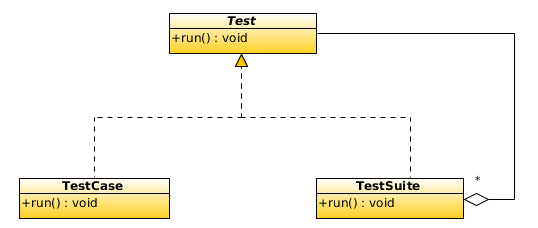
\includegraphics[width=0.8\textwidth]{figures/xunit/test-tree.png}
\caption{组合:构建隐式树}
 \label{fig:test-tree}
\end{figure}

\section{命名用例}

可以给每个\ascii{TestCase, TestSuite}命名,方便后期用例的定位与调试。

\subsection{测试用例}

\begin{nodiff}{test/mars/core/TestCaseSpec.cc}
 \begin{c++}
#include <gtest/gtest.h>
#include "mars/core/TestCase.h"

namespace {
  void assertName(const Test& test, const char* expected) {
    ASSERT_EQ(std::string(expected), test.getName());
  }
}

TEST(NamedTestCase, named_test_case) {
  assertName(TestCase("test case1"), "test case1");
}
 \end{c++}
\end{nodiff}

\subsection{通过测试}

首先,增加抽象接口\ascii{Test::getName}。

\begin{diff}{include/mars/core/Test.h}
 \begin{minicpp}
#include <string>

struct Test {
  virtual void run() = 0;
  
  virtual ~Test() {}
};
 \end{minicpp}
 \tcblower
 \begin{minicpp}
#include <string>

struct Test {
  virtual void run() = 0;
  virtual const std::string& getName() const = 0;

  virtual ~Test() {}
};
 \end{minicpp}
\end{diff}

在\ascii{TestCase}中覆写\ascii{getName}成员函数。其中,为默认构造函数提供空字符串,保证既有的用例都能通过。

\begin{diff}{include/mars/core/TestCase.h}
 \begin{minicpp}
#include "mars/core/Test.h"

struct TestCase : Test {
private:
  void run() override;

private:
  virtual void setUp() {}
  virtual void runTest() {}
  virtual void tearDown() {}
};
 \end{minicpp}
\tcblower
 \begin{minicpp}
#include "mars/core/Test.h"

struct TestCase : Test {
  explicit TestCase(const std::string& = "");

private:
  void run() override;
  const std::string& getName() const override;

private:
  virtual void setUp() {}
  virtual void runTest() {}
  virtual void tearDown() {}

private:
  std::string name;
};
 \end{minicpp}
\end{diff}

在\ascii{TestCase.cc}中实现,也极为简单。

\begin{diff}{src/mars/core/TestCase.cc}
 \begin{minicpp}
#include "mars/core/TestCase.h"

void TestCase::run() {
  setUp();
  runTest();
  tearDown();
}
 \end{minicpp}
\tcblower
 \begin{minicpp}
#include "mars/core/TestCase.h"

void TestCase::run() {
  setUp();
  runTest();
  tearDown();
}

TestCase::TestCase(const std::string& name)
  : name(name) {
}

const std::string& TestCase::getName() const {
  return name;
}
 \end{minicpp}
\end{diff}

依葫芦画瓢,\ascii{TestSuite}的名字实现与\ascii{TestCase}雷同。

\begin{diff}{include/mars/core/TestSuite.h}
 \begin{minicpp}
#include <vector>
#include "mars/core/Test.h"

struct TestSuite : Test {
  ~TestSuite();
  void add(Test* test);

private:
  void run() override;

private:
  template <typename F>
  void foreach(F f) const;

private:
  std::vector<Test*> tests;
};
 \end{minicpp}
\tcblower
 \begin{minicpp}
#include <vector>
#include "mars/core/Test.h"

struct TestSuite : Test {
  explicit TestSuite(const std::string& = "");
  ~TestSuite();

  void add(Test* test);

private:
  const std::string& getName() const override;
  void run() override;

private:
  template <typename F>
  void foreach(F f) const;

private:
  std::string name;
  std::vector<Test*> tests;
};
 \end{minicpp}
\end{diff}

在实现文件中,实现相关成员函数。

\begin{diff}{src/mars/core/TestSuite.cc}
 \begin{minicpp}
#include "mars/core/TestSuite.h"

void TestSuite::add(Test* test) {
  tests.push_back(test);
}

template <typename F>
inline void TestSuite::foreach(F f) const {
  for (auto test : tests) {
    f(test);
  }
}

TestSuite::~TestSuite() {
  foreach([](auto test) {
    delete test;
  });
}

void TestSuite::run() {
  foreach([](auto test) {
    test->run();
  });
}
 \end{minicpp}
\tcblower
 \begin{minicpp}
#include "mars/core/TestSuite.h"

void TestSuite::add(Test* test) {
  tests.push_back(test);
}

template <typename F>
inline void TestSuite::foreach(F f) const {
  for (auto test : tests) {
    f(test);
  }
}

TestSuite::~TestSuite() {
  foreach([](auto test) {
    delete test;
  });
}

void TestSuite::run() {
  foreach([](auto test) {
    test->run();
  });
}

TestSuite::TestSuite(const std::string& name)
  : name(name) {
}

const std::string& TestSuite::getName() const {
  return name;
}
 \end{minicpp}
\end{diff}

至此,测试通过。

\subsection{消除重复}

但是,\ascii{TestCase}与\ascii{TestSuite}存在结构性重复设计,包括相同的构造函数,覆写\ascii{getName}成员函数,私有字段\ascii{name}。为了消除重复,重构将公共实现搬迁至父类。

搬迁至父类需要关注两点:

\begin{enum}
  \eitem{\ascii{Test}的构造函数被声明为\ascii{public},方便子类使用\ascii{using}语句直接复用构造函数。}
  \eitem{\ascii{getName}没有必要声明为虚函数,因为在\ascii{Test}内已经完全具备实现的条件;子类强制继承\ascii{getName}的实现,拒绝被覆写。}
\end{enum}

\begin{diff}{include/mars/core/Test.h}
 \begin{minicpp}
#include <string>

struct Test {
  virtual void run() = 0;
  virtual const std::string& getName() const = 0;

  virtual ~Test() {}
};
 \end{minicpp}
\tcblower
 \begin{minicpp}
#include <string>

struct Test {
  explicit Test(const std::string& name = "");
  const std::string& getName() const;

  virtual void run() = 0;
  virtual ~Test() {}

private:
  std::string name;
};
 \end{minicpp}
\end{diff}

\ascii{Test::getName}实现异常简单。

\begin{nodiff}{src/mars/core/Test.cc}
 \begin{c++}
#include "mars/core/Test.h"

Test::Test(const std::string& name)
  : name(name) {}

const std::string& Test::getName() const {
  return name;
}
 \end{c++}
\end{nodiff}

在\ascii{TestCase}中,直接使用\ascii{using}语句复用构造函数,删除既有的\ascii{TestCase::getName}实现,及其私有字段\ascii{std::string name}。

\begin{diff}{include/mars/core/TestCase.h}
 \begin{minicpp}
#include "mars/core/Test.h"

struct TestCase : Test {
  explicit TestCase(const std::string& = "");

private:
  const std::string& getName() const override;
  void run() override;

private:
  virtual void setUp() {}
  virtual void runTest() {}
  virtual void tearDown() {}
};
 \end{minicpp}
\tcblower
 \begin{minicpp}
#include "mars/core/Test.h"

struct TestCase : Test {
  using Test::Test;

private:
  void run() override;

private:
  virtual void setUp() {}
  virtual void runTest() {}
  virtual void tearDown() {}
};
 \end{minicpp}
\end{diff}

同理,\ascii{TestSuite}中通过相同的手段实现代码复用。

\begin{diff}{include/mars/core/TestSuite.h}
 \begin{minicpp}
#include <vector>
#include "mars/core/Test.h"

struct TestSuite : Test {
  explicit TestSuite(const std::string& = "");
  ~TestSuite();subsection

  void add(Testsubsection

private:
  const std::string& getName() const override;
  void run() override;

private:
  template <typename F>
  void foreach(F f) const;

private:
  std::string name;
  std::vector<Test*> tests;
};
 \end{minicpp}
\tcblower
 \begin{minicpp}
#include <vector>
#include "mars/core/Test.h"

struct TestSuite : Test {
  using Test::Test;

  ~TestSuite();subsection

  void add(Testsubsection

private:
  void run() override;

private:
  template <typename F>
  void foreach(F f) const;

private:
  std::vector<Test*> tests;
};
 \end{minicpp}
\end{diff}

遗憾的是,\ascii{Test}构造函数未能声明为\ascii{protected}。但是,即使\ascii{Test}的构造函数虽然被声明为\ascii{public},设计并未丢失编译时的安全检查。因为\ascii{Test::run}被声明为纯虚函数,在编译时保证用户无法直接创建\ascii{Test}实例。

\end{content}

